% !BIB TS-program = biber
% !BIB program = biber
\documentclass[times]{itmo-student-thesis}

%% Опции пакета:
%% - specification - если есть, генерируется задание, иначе не генерируется
%% - annotation - если есть, генерируется аннотация, иначе не генерируется
%% - times - делает все шрифтом Times New Roman, собирается с помощью xelatex
%% - languages={...} - устанавливает перечень используемых языков. По умолчанию это {english,russian}.
%%                     Последний из языков определяет текст основного документа.

\usepackage{graphicx}
\graphicspath{ {./img/} }

%% Делает запятую в формулах более интеллектуальной, например:
%% $1,5x$ будет читаться как полтора икса, а не один запятая пять иксов.
%% Однако если написать $1, 5x$, то все будет как прежде.
\usepackage{icomma}

%% Один из пакетов, позволяющий делать таблицы на всю ширину текста.
\usepackage{tabularx}

%% Данные пакеты необязательны к использованию в бакалаврских/магистерских
%% Они нужны для иллюстративных целей
%% Начало
\usepackage{tikz}
\usetikzlibrary{arrows}
\usepackage{filecontents}
\begin{filecontents}{master-thesis.bib}

@online{ programmatic-buying,
    title = {Programmatic Buying - Definition and Demarcation},
    url = {https://en.ryte.com/wiki/Programmatic_Buying},
    langid = {english},
    urldate = {2020-05-26},
    year = {2020}
}

@online{ growth-of-programmatic,
    title = {How is programmatic marketing and digital display advertising defined},
    url = {https://www.smartinsights.com/internet-advertising/internet-advertising-targeting/what-is-programmatic-marketing/},
    langid = {english},
    urldate = {2020-05-26},
    year = {2020}
}

@online{ ad-server,
    title = {Ad serving},
    url = {https://en.wikipedia.org/wiki/Ad_serving},
    langid = {english},
    urldate = {2020-05-26},
    year = {2020}
}

@online{ three-tier-architecture,
    title = {Three-tier architecture},
    url = {https://en.wikipedia.org/wiki/Multitier_architecture#Three-tier_architecture},
    langid = {english},
    urldate = {2020-05-26},
    year = {2020}
}

@online{ data-access-layer,
    title = {Data access layer},
    url = {https://en.wikipedia.org/wiki/Data_access_layer},
    langid = {english},
    urldate = {2020-05-26},
    year = {2020}
}

@online{ twelve-factor-app,
    title = {The Twelve-Factor App},
    url = {https://12factor.net/},
    langid = {english},
    urldate = {2020-05-26},
    year = {2020}
}

@online{ mongodb,
    title = {The most popular database for modern apps | MongoDB},
    url = {https://www.mongodb.com/},
    langid = {english},
    urldate = {2020-05-26},
    year = {2020}
}

@online{ amazon-paapi-docs,
    title = {Product Advertising API 5.0 - documentation},
    url = {https://webservices.amazon.com/paapi5/documentation/},
    langid = {english},
    urldate = {2020-05-26},
    year = {2020}
}

@online{ amazon-paapi-sdk,
    title = {Product Advertising API 5.0 - Node.js SDK},
    url = {https://webservices.amazon.com/paapi5/documentation/assets/archives/paapi5-nodejs-sdk-example.zip},
    langid = {english},
    urldate = {2020-05-26},
    year = {2020}
}

@online{ repository-pattern,
    title = {Repository Pattern},
    url = {https://deviq.com/repository-pattern/},
    langid = {english},
    urldate = {2020-05-26},
    year = {2020}
}

@online{ typescript-lang,
    title = {TypeScript - JavaScript that scales.},
    url = {https://www.typescriptlang.org/},
    langid = {english},
    urldate = {2020-05-26},
    year = {2020}
}

@online{ contextual-targeting,
    title = {Contextual advertising},
    url = {https://en.wikipedia.org/wiki/Contextual_advertising},
    langid = {english},
    urldate = {2020-05-26},
    year = {2020}
}

@online{ behavioural-targeting,
    title = {Behavioural targeting},
    url = {https://en.wikipedia.org/wiki/Targeted_advertising#Behavioural_targeting},
    langid = {english},
    urldate = {2020-05-26},
    year = {2020}
}

@online{ creative-sequencing,
    title = {Creative sequencing},
    url = {https://en.wikipedia.org/wiki/Creative_sequencing},
    langid = {english},
    urldate = {2020-05-26},
    year = {2020}
}

@online{ SOLID,
    title = {SOLID},
    url = {https://en.wikipedia.org/wiki/SOLID},
    langid = {english},
    urldate = {2020-05-26},
    year = {2020}
}

@online{ capterra,
    title = {Capterra - find the best Ad Server Software for your business},
    url = {https://www.capterra.com/ad-server-software/},
    langid = {english},
    urldate = {2020-05-26},
    year = {2020}
}

@online{ revive-adserver,
    title = {Free Open Source Ad Server - Revive Adserver},
    url = {https://www.revive-adserver.net/},
    langid = {english},
    urldate = {2020-05-26},
    year = {2020}
}

@online{ google-ad-manager,
    title = {Google Ad Manager},
    url = {https://admanager.google.com/home/},
    langid = {english},
    urldate = {2020-05-26},
    year = {2020}
}

@online{ adzerk,
    title = {Build an Ad Server in Weeks | Adzerk},
    url = {https://adzerk.com/},
    langid = {english},
    urldate = {2020-05-26},
    year = {2020}
}

@online{ epom-ad-server,
    title = {Epom Ad Server | Leading Ad Serving Platform for Networks},
    url = {https://epom.com/},
    langid = {english},
    urldate = {2020-05-26},
    year = {2020}
}

@online{ mopub,
    title = {Powerful app monetization | MoPub},
    url = {https://www.mopub.com/en},
    langid = {english},
    urldate = {2020-05-26},
    year = {2020}
}

\end{filecontents}
%% Конец

%% Указываем файл с библиографией.
\addbibresource{master-thesis.bib}

%% Добавляем подсветку синтаксиса для ECMAScript 6
\usepackage{listings}
\usepackage{color}
\usepackage{textcomp} % for upquote

%
% ECMAScript 2015 (ES6) definition by Gary Hammock
%

\lstdefinelanguage[ECMAScript2015]{JavaScript}[]{JavaScript}{
  morekeywords=[1]{await, async, case, catch, class, const, default, do,
    enum, export, extends, finally, from, implements, import, instanceof,
    let, static, super, switch, throw, try, public, constructor},
  morestring=[b]` % Interpolation strings.
}


%
% JavaScript version 1.1 by Gary Hammock
%
% Reference:
%   B. Eich and C. Rand Mckinney, "JavaScript Language Specification
%     (Preliminary Draft)", JavaScript 1.1.  1996-11-18.  [Online]
%     http://hepunx.rl.ac.uk/~adye/jsspec11/titlepg2.htm
%

\lstdefinelanguage{JavaScript}{
  morekeywords=[1]{break, continue, delete, else, for, function, if, in,
    new, return, this, typeof, var, void, while, with},
  % Literals, primitive types, and reference types.
  morekeywords=[2]{false, null, true, boolean, number, undefined,
    Array, Boolean, Date, Math, Number, String, Object},
  % Built-ins.
  morekeywords=[3]{eval, parseInt, parseFloat, escape, unescape},
  sensitive,
  morecomment=[s]{/*}{*/},
  morecomment=[l]//,
  morecomment=[s]{/**}{*/}, % JavaDoc style comments
  morestring=[b]',
  morestring=[b]"
}[keywords, comments, strings]


\lstalias[]{ES6}[ECMAScript2015]{JavaScript}

% Requires package: color.
\definecolor{mediumgray}{rgb}{0.3, 0.4, 0.4}
\definecolor{mediumblue}{rgb}{0.0, 0.0, 0.8}
\definecolor{forestgreen}{rgb}{0.13, 0.55, 0.13}
\definecolor{darkviolet}{rgb}{0.58, 0.0, 0.83}
\definecolor{royalblue}{rgb}{0.25, 0.41, 0.88}
\definecolor{crimson}{rgb}{0.86, 0.8, 0.24}

\lstdefinestyle{JSES6Base}{
  backgroundcolor=\color{white},
  basicstyle=\ttfamily,
  breakatwhitespace=false,
  breaklines=false,
  captionpos=b,
  columns=fullflexible,
  commentstyle=\color{mediumgray}\upshape,
  emph={},
  emphstyle=\color{crimson},
  extendedchars=true,  % requires inputenc
  fontadjust=true,
  frame=single,
  identifierstyle=\color{black},
  keepspaces=true,
  keywordstyle=\color{mediumblue},
  keywordstyle={[2]\color{darkviolet}},
  keywordstyle={[3]\color{royalblue}},
  numbers=left,
  numbersep=5pt,
  numberstyle=\tiny\color{black},
  rulecolor=\color{black},
  showlines=true,
  showspaces=false,
  showstringspaces=false,
  showtabs=false,
  stringstyle=\color{forestgreen},
  tabsize=2,
  title=\lstname,
  upquote=true  % requires textcomp
}

\lstdefinestyle{JavaScript}{
  language=JavaScript,
  style=JSES6Base
}
\lstdefinestyle{ES6}{
  language=ES6,
  style=JSES6Base
}

\begin{document}

\studygroup{M42381}
\title{Разработка платформы для управления
таргетированной рекламой}
\author{Чекменев Александр Романович}{Чекменев А.Р.}
\supervisor{Фильченков Андрей Александович}{Фильченков А. А.}{к.ф.-м.н.}{доц. ФИТиП}
\publishyear{2020}
%% Дата выдачи задания. Можно не указывать, тогда надо будет заполнить от руки.
\startdate{01}{сентября}{2019}
%% Срок сдачи студентом работы. Можно не указывать, тогда надо будет заполнить от руки.
%\finishdate{31}{мая}{2020}
%% Дата защиты. Можно не указывать, тогда надо будет заполнить от руки.
%\defencedate{15}{июня}{2019}

%\addconsultant{Белашенков Н.Р.}{канд. физ.-мат. наук, без звания}
%\addconsultant{Беззубик В.В.}{без степени, без звания}

\secretary{Павлова О.Н.}

%% Задание
%%% Техническое задание и исходные данные к работе
\technicalspec{Требуется разработать программное обеспечение, обеспечивающее работу требуемых функций рекламной сети согласно установленным требованиям.}

%%% Содержание выпускной квалификационной работы (перечень подлежащих разработке вопросов)
\plannedcontents{}

%%% Исходные материалы и пособия 
\plannedsources{\begin{enumerate}
    \item 
\end{enumerate}}

%%% Цель исследования
\researchaim{}

%%% Задачи, решаемые в ВКР
\researchtargets{\begin{enumerate}
    \item разработка рекламной сети
\end{enumerate}}

%%% Использование современных пакетов компьютерных программ и технологий

%%% Краткая характеристика полученных результатов 
\researchsummary{Рекламная сеть запущена в production-окружении платформы Google Kubernetes Cloud. Примеры рекламных объявлений различного формата доступны в приложении Fulldive Browser на платформе Android.}

%%% Гранты, полученные при выполнении работы 
\researchfunding{}

%%% Наличие публикаций и выступлений на конференциях по теме выпускной работы
\researchpublications{}

%% Эта команда генерирует титульный лист и аннотацию.
\maketitle{Магистр}

%% Оглавление
\tableofcontents





%% Макрос для введения. Совместим со старым стилевиком.

\startprefacepage

Прогресс в сфере технологий и интеллектуальных систем неизбежно влечет за собой активное развитие всех смежных областей, а достижения вследствие такого развития внедряются и в другие сферы. Сфера digital-рекламы в этом плане не является исключением. 

Результатом применения современных подходов в digital-рекламе является, например, алгоритмическая закупка рекламы (англ. programmatic buying) \cite{programmatic-buying} — способ закупки целевого трафика с оплатой за совершенные целевые действия. Данный способ активно вытесняет традиционные способы закупки рекламы, так как обладает рядом преимуществ. Например, позволяет в режиме реального времени за долю секунды подобрать специальное рекламное объявление для каждого конкретного пользователя с учетом его демографических данных, места жительства, интересов и прочих параметров. По прогнозам маркетинговых агентств в 2020 году 69\% digital-рекламы будет закуплено программно \cite{growth-of-programmatic}. 

Одной из причин столь активного вытеснения ранее существующих подхов стало повышение эффективности алгоритмов таргетинга. 

\begin{figure}[!h]
\caption{Рост доли алгоритмической закупки рекламы}\label{fig:share-of-programmatic}
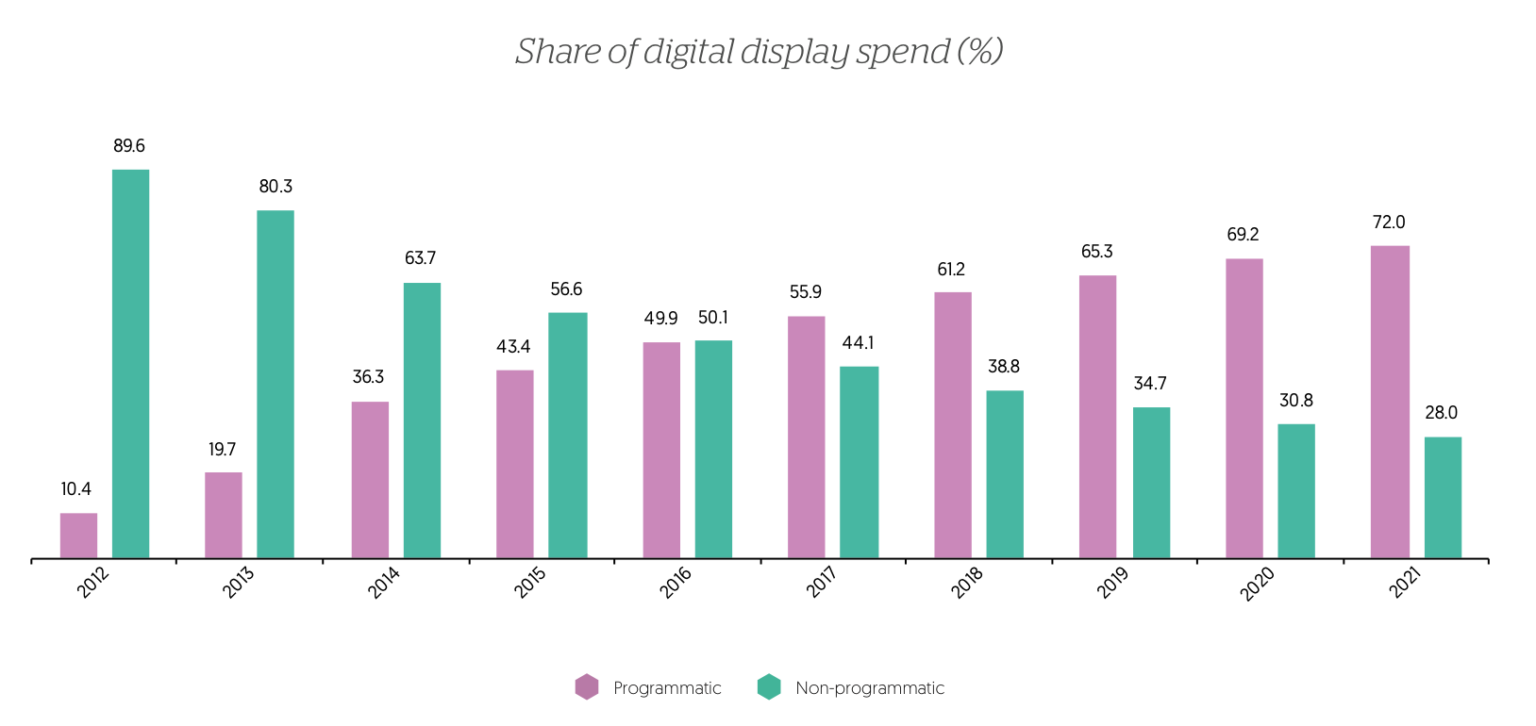
\includegraphics[width=\textwidth]{share-of-programmatic}
\centering
\end{figure}

В данный момент таргетированная реклама одна из наиболее развивающихся областей digital-рекламы, так как позволяет максимально гибко и точно задать необходимую целевую аудиторию для каждого рекламного объявления. Существует ряд компаний, предоставляющих услуги по размещению таргетированной рекламы в своих рекламных сетях. Но все они имеют такие существенные недостатки, как отсутствие прямого доступа к целевой аудитории, а также строгая зависимость от условий, устанавливаемых рекламными площадками. Все это создает трудности в воплощении нестандартных подходов для компаний, которые по каким-либо причинам не могут выполнить установленные требования, и дает все основания задуматься о создании собственной рекламной сети.

Компания Fulldive разработала приложение Fulldive VR, которое входит в топ-5 приложений для Android в категории VR. Fulldive Browser — второй и активно развивающийся продукт компании. Одним из его выжнейших и эффективно влияющих на привлечение новых пользователей преимуществом является возможность пользователя монетизировать свое время, проведенное за чтением новостей, общением в социальных сетях, просмотром роликов и другими действиями, типично совершаемыми в любом другом браузере. Достигается это за счет того, что компания отдает пользователю часть прибыли, полученной от рекламных сетей за просмотры рекламы, совершенные пользователем приложении. 

Далеко не все рекламные площадки приветствуют такой способ мотивации пользователей, но реализация рекламы внутри своих приложений с использованием собственной рекламной сети поможет избежать данной проблемы. Это позволит компании в полной мере следовать своей стратегии развития не боясь сокращения или потери доходов от рекламы в будущем, а также позволит не отдавать часть прибыли сторонним рекламным площадкам.

Таким образом, можно выделить следующие преимущества наличия у компании собственной рекламной сети:
\begin{enumerate}
	\item диверсификация риска сокращения прибыли от рекламы из-за прекращения сотрудничества с основными рекламными сетями;
	\item возможность добавления собственных рекламных форматов;
	\item возможность более тонко настраивать где и в каком контексте будет показана реклама;
	\item возможность сбора данных непосредственного взаимодействия пользователей с рекламой (First-Party Data), которые представляет наивысшую ценность, так как является наиболее точными, качественными и принадлежат компании;
	\item возможность использования собственной рекламной сети для привлечения сторонних рекламодателей.
\end{enumerate}

Целью данной работы является создание собственной рекламной сети UniAds, для функционирования которой необходимо разработать рекламный сервер на основе установленных бизнес-требований.

В первой главе приводится список используемых терминов, формулируется цель и постановка решаемой задачи, рассматриваются существующие решения. В второй главе приводится архитектура предлагаемого решения поставленной задачи. В третьей главе рассматриваются аспекты, связанные с технической реализацией приведенного во второй главе решения. В заключении приводятся полученные результаты, подводятся итоги проделанной работы и предлагаются направления для дальнейшей деятельности.




%% Начало содержательной части.

\chapter{Постановка задачи и обзор существующих реализаций рекламного сервера}\label{chapter:1}

\startrelatedwork %% Так помечается начало обзора.

В начале данной главы приведены определения для основных терминов и понятий, используемых в работе. Затем формулируются цель работы, постановка задачи с разбиением на необходимые подзадачи и требования к результатам проделанной работы. В конце главы проводится обзор существующих решений, удовлетворяющих сформулированным требованиям.

\section{Используемые термины и понятия}\label{sec:terms}

\subsection{Рекламная сеть}

\textbf{Рекламная сеть} (англ. ad network)\label{ad-network} — это технологическая платформа, которая обеспечивает продажи рекламных ресурсов между издателями и рекламодателями. Ключевой функцией рекламной сети является агрегация рекламного предложения от издателей и его соответствие спросу рекламодателя. Принципиальное различие между традиционными рекламными сетями в средствах массовой информации и рекламными сетями в интернете заключается в том, что рекламные сети в интернете используют рекламные серверы для таргетирования и доставки рекламы потребителям, отслеживания и составления отчетов о показах способами, невозможными при использовании аналоговых средств массовой информации.

\textbf{Таргетированная рекламная сеть} (англ. targeted ad network) — наиболее продвинутый вид рекламных сетей, которые специализируются на технологиях точного таргетирования по поведенческим или контекстным признакам, активно анализируют данные о пользователях в целях повышения стоимости инвентаря, который они продают.

\subsection{Рекламодатель}

\textbf{Рекламодатель} (англ. advertiser) — участник рекламной сети, который управляет и оплачивает рекламу продукта или услуги и, фактически, представляющий сторону спроса. 

Рекламодатель как пользователь рекламной сети:
\begin{itemize}
\item создает рекламные материалы различных форматов;
\item выбирает модель оплаты и согласно ей оплачивает приобретенные у издателя ресурсы;
\item конфигурирует целевую аудиторию для каждого управляемого им рекламного объявления;
\item управляет категориями подходящих рекламных площадок и издателей.
\end{itemize}

\subsection{Издатель}

\textbf{Издатель} (англ. publisher) — владелец рекламной площадки, на которой рекламодатель размещает свою рекламу. За данную услугу издатель взимает с рекламодателя определенную сумму в соответствии с одной из ценовых моделей размещения рекламы. Чаще всего рекламной площадкой является веб-сайт или мобильное приложение.

Издатель как пользователь рекламной сети:
\begin{itemize}
\item регистрирует рекламную площадку и указывает ее параметры: тематику, тип и объем доступной аудитории и т.д.;
\item создает элементы рекламного инвентаря, которые будут использованы для продажи рекламодателям доступные для показа рекламы места;
\item управляет категориями допустимых рекламодателей.
\end{itemize}

\subsection{Рекламный сервер}

\textbf{Рекламный сервер} (англ. ad server) \cite{ad-server} — это технологическая платформа (обычно веб-ориентированная), отвечающая за размещение, оптимизацию и распространение рекламного контента на различных веб-сайтах и в мобильных приложениях. Рекламные серверы также отвечают за управление и отслеживание рекламы, составление отчетов и выставление счетов рекламодателям.

\textbf{Показ рекламы} (англ. ad serving)\label{ad-serving} — это технологический цикл, в котором рекламный сервер используется для размещения рекламы на различных веб-сайтах и в мобильных приложениях. Механизм показа рекламы является ключевым элементом каждого рекламного сервера. Он использует сложные алгоритмы и передовые инструменты принятия решений для выбора наиболее релевантной рекламы для показа. Процесс выбора рекламы строго ограничен правилами, которые определены издателями, рекламодателями и самим рекламным сервером. Эти правила включают критерии таргетинга, частоту просмотра, место размещения рекламы, приоритет рекламы, потенциальный доход и другие параметры. 

Рекламный сервер должен учитывать все эти факторы в режиме реального времени и возвращать результат в течение миллисекунд. Любая задержка приведет к дополнительным задержкам при загрузке страницы, что приведет к меньшему количеству просмотров страниц  и показов рекламы.

Существует два типа рекламных серверов: один — для рекламодателей, другой — для издателей (рекламных площадок). Их отличие заключается в организации данных и удобстве работы для каждой группы пользователей.

Рекламодатели используют единый сервер объявлений, где хранится рекламный контент и предоставляется функционал для отчетов по показам, кликам и другим метрикам. Такой централизованный сервис, контролирующий распространение контента на сайтах, делает удобным отслеживание и управление рекламными материалами, повышает точность таргетинга.

Издатели — владельцы площадок — имеют отдельные рекламные серверы (только для своих доменов). Это удобно, поскольку у них есть доступ только к тому рекламному контенту, который требуется для публикации, и не нужно фильтровать все рекламные материалы на централизованном сервере.

\subsection{Таргетинг}

\textbf{Таргетинг} (англ. ad targeting)\label{targeting} — рекламный механизм, позволяющий выделить из всей имеющейся аудитории только ту часть, которая удовлетворяет заданным критериям (целевую аудиторию), и показать конкретное объявление именно ей.

Цель таргетинга — создать рекламно-информационное сообщение, по своей форме и содержанию максимально ориентированное на заинтересованную в конкретном товаре/услуге части аудитории, а также повысить эффективность взаимодействия с этой аудиторией и получить как можно большей отдачи от неё.

Преимущества таргетинга:
\begin{itemize}
\item возможность выделить ту аудиторию, заинтересованную в покупке товара или услуги
\item возможность снизить расходы на рекламу за счёт правильного выбора таргетинга для целевой аудитории
\item возможность разделить всю целевую аудиторию  на группы и для каждой группы сформировать уникальное предложение
\end{itemize}

В зависимости от того на основе какой информации принимается решение о выборе объявления выделяют такие виды таргетинга, как контекстный и поведенческий.

\textbf{Контекстный таргетинг} (англ. contextual targeting)\cite{contextual-targeting} — это практика показа рекламы на основе содержания веб-сайта. Существует контекстный таргетинг на категории, где объявления ориентированы на страницы, которые попадают в предварительно назначенные категории, и контекстный таргетинг на ключевые слова, где объявления ориентированы на страницы, соответствующие определенным ключевым словам. 

Семантический таргетинг является наиболее эффективной формой контекстного таргетинга. Он предполагает использование машинного обучения для распознавания контекста и семантики каждой страницы, содержащей определенный контент, а не просто определение подходящих ключевых слов на странице. Когда пользователь заходит на страницу, информация о содержимом этой веб-страницы попадает на рекламный сервер, который затем сопоставляет ее с релевантными объявлениями по ключевым словам и содержанию. Чем лучше система понимает контекст страницы, тем релевантнее будет реклама.

\textbf{Поведенческий таргетинг} (англ. behavioral targeting)\label{behavioral-targeting} — это практика сегментирования клиентов на основе поведения при просмотре веб-страниц или действий в мобильном приложении. 

Данные о поведении пользователя служат для:
\begin{itemize}
\item показа релевантной, персонализированной рекламы в тот момент, когда покупатель, скорее всего, совершит покупку
\item изучения интересов, предпочтений и планов потенциальных покупателей
\item формирования портретов разных сегментов целевой аудитории
\item повышения лояльности к продукту и отклика на рекламу
\item расширения целевой аудитории
\end{itemize}

Поведенческий таргетинг позволяет показывать объявления пользователям, которые действительно заинтересованы в рекламируемом товаре или услуге. Обратиться к целевой аудитории можно даже на тех страницах, содержание которых не соответствует тематике объявления.

\subsection{Трекинг}

\textbf{Трекинг} (англ. ad tracking) или отслеживание рекламы — фиксация различных событий взаимодействия пользователя с рекламой. Данными событиями, например, являются показы, клики и конверсии. Все они записываются в базу данных для дальнейшей обработки и анализа. Процесс отслеживания рекламы важен, так как помогает измерить и оценить каждое объявление по его эффективности.

\textbf{Конверсионная воронка}  — это последовательность совершенных на сайте пользователем действий (микроконверсий), ведущих его к конечной цели (макроконверсии), визуализированная в виде воронки, т.к. достижение каждой следующей микроконверсии в количественном выражении меньше, чем достижения предыдущей. В зависимости от того влияют ли результаты предыдущих стадий на последующие, воронки могут быть одного из двух типов: открытые или закрытые.

Метрики — параметры, рассчитываемые на основе данных трекинга. На основе таких параметров проводится прогнозирование и анализ эффективности рекламных кампаний. 

Метрики используемые в данной работе:
\begin{itemize}
\item OR (англ. open rate) — отношение числа показов рекламы к числу запросов рекламных объявлений
\item CTR (англ. click-through rate) — отношение числа кликов на рекламное объявление к числу показов
\item CPA (англ. cost per action) — отношение общей стоимости рекламы к количеству совершенных целевых действий; стоимость целевого действия
\end{itemize}

\subsection{Микросервисная архитектура}

\textbf{Микросервисная архитектура} — вариант сервис-ориентированной архитектуры программного обеспечения, направленный на взаимодействие насколько это возможно небольших, слабо связанных и легко изменяемых модулей — микросервисов, получивший распространение в середине 2010-х годов в связи с развитием практик гибкой разработки и DevOps.

Свойства, характерные для микросервисной архитектуры:
\begin{itemize}
\item модули можно легко заменить в любое время: акцент на простоту, независимость развёртывания и обновления каждого из микросервисов;
\item модули организованы вокруг функций: микросервис по возможности выполняет только одну достаточно элементарную функцию;
\item модули могут быть реализованы с использованием различных языков программирования, фреймворков, связующего программного обеспечения, выполняться в различных средах контейнеризации, виртуализации, под управлением различных операционных систем на различных аппаратных платформах: приоритет отдаётся в пользу наибольшей эффективности для каждой конкретной функции, нежели стандартизации средств разработки и исполнения;
\item архитектура симметричная, а не иерархическая: зависимости между микросервисами одноранговые.
\end{itemize}


\subsection{Трехуровневая архитектура}

\textbf{Трёхуровневая архитектура} (англ. three-tier) — архитектурная модель программного комплекса, предполагающая наличие в нём трёх компонентов: клиента, сервера приложений (к которому подключено клиентское приложение) и сервера баз данных (с которым работает сервер приложений).

Клиент (слой клиента) — это интерфейсный компонент комплекса, предоставляемый конечному пользователю. Этот уровень не должен иметь прямых связей с базой данных, быть нагруженным основной бизнес-логикой и хранить состояние приложения. На этот уровень обычно выносится только простейшая бизнес-логика.

Сервер приложений (средний слой, связующий слой) располагается на втором уровне, на нём сосредоточена большая часть бизнес-логики. Серверы приложений проектируются таким образом, чтобы добавление к ним дополнительных экземпляров обеспечивало горизонтальное масштабирование производительности программного комплекса и не требовало внесения изменений в программный код приложения.

Сервер баз данных (слой данных) обеспечивает хранение данных и выносится на отдельный уровень, реализуется, как правило, средствами систем управления базами данных, подключение к этому компоненту обеспечивается только с уровня сервера приложений.

% \subsection{Node.js}

% TODO

% \subsection{Развертывание}

% Google Cloud

% Google Container Registry

% Kubernetes

% Docker




\section{Постановка задачи}

Fulldive Browser — браузер, который помимо втроенных возможностей социальных сетей позволяет пользователям получать часть дохода компании от просмотренной рекламы. В приложении используется таргетированная реклама, закупаемая у сторонних рекламных сетей, таких как Google AdMob, Facebook Audience Network, MoPub, PubMatic и других. Практически каждая из приведенных рекламных сетей либо запрещает возвращать часть доходов пользователям приложения, либо накладывает существенные ограничения на объем и качество поставляемой рекламы. Подобные ограничения являются вполне обоснованным решением для создания собственной рекламной сети.

Целью данной работы является создание собственной рекламной сети UniAds, для функционирования которой необходимо разработать рекламный сервер на основе установленных бизнес-требований.

Разработка рекламного сервера \ref{ad-server} сводится к решению следующих подзадач:
\begin{itemize}
\item разработка контракта клиент-серверного взаимодействия;
\item разработка архитектуры серверного приложения;
\item разработка модуля для создания и обновления рекламных объявлений на основе товаров Amazon;
\item разработка механизма получения списка объявлений с сохранением консистентности;
\item разработка алгоритмов работы стратегий таргетирования объявлений;
\item разработка системы трекинга просмотров и переходов по объявлениям, с возможностью просмотра статистики по объявлениям и стратегиям таргетинга.
\end{itemize}

Каждая из позадач подразумевает составление требований, разработку архитектуры необходимых модулей и их взаимодействия, программную реализацию, соответствующее тестирование полученных модулей и внедрение. 

Основнымм требованиями к рекламному серверу является возможность непосредственного доступа сотрудников компании для модификации исходного кода сервера, возможность развертывания в контроллируемом окружении в облачной инфраструктуре Google Cloud, а также желательно использование платформы Node.js при реализации сервера. Требования к каждому отдельному модулю приводятся в в описании соответствующего модуля.

\section{Обзор существующих решений}

Для применения наиболее эффективных и актуальных подходов при решении приведенных подзадач рассмотрим наиболее эффективные и популярные (по рейтингу Capterra \cite{capterra}) существующие реализации функционала рекламного сервера.


Revive Adserver \cite{revive-adserver} — единственная open-source реализация на языке PHP, разработанная много лет назад в компании OpenX. Данный продукт хорошо подходит компаниям, которые:
\begin{itemize}
\item не хотят платить ежемесечную абонентскую плату за использование продукта;
\item обладают собственными инженерными ресурсами;
\item хотят существенно сэкономить ресурсы на разработку собственного решения.
\end{itemize}
И в то же время данный продукт:
\begin{itemize}
\item согласно документации не позволяет использовать собственные алгоритмы таргетинга;
\item обладает слабой гибкостью в использовании собственных рекламных форматов;
\item обладает очень скудной и местами устаревшей документаций, что затрудняет процесс интеграции данного решения в экосистему компании.
\end{itemize}


В июне 2018 года Google объявила о новом брендинге для ряда своих рекламных продуктов. Благодаря этой инициативе они объединили свой рекламный сервер DoubleClick For Publishers со своей биржей рекламы Google Ad Exchange в единую платформу под названием Google Ad Manager (GAM) \cite{google-ad-manager}. Этот инструмент призван помочь как рекламодателям, так и издателям оптимизировать процесс показа рекламы, позволяя брендам управлять рекламой и доставлять ее в различные аудитории с одной платформы. 

Данный инструмент обладает такими преимуществами как высокая степень отказоустойчивости, тесная взаимосвязь с другими сервисами компании Google и подробная документация. Но в то же время его существенными недостатками являются:
\begin{itemize}
\item размещение на серверах компании Google без доступа к исходному коду;
\item низкий уровень гибкости форматов рекламных объявлений
\item существенная ограниченность в применении собственных алгоритмов таргетинга
\item пользовательские данные хранятся на серверах Google
\end{itemize}


Adzerk\cite{adzerk} - это облачная платформа для разработки рекламных серверов. Платформа предлагает различные API для облегчения проектирования, разработки и развертывания всех видов рекламных серверов. Adzerk включает в себя несколько систем управления базами данных, таких как UserDB и ContentDB, чтобы помочь пользователям управлять ограничением частоты, поведенческим таргетингом, таргетингом на страницы, динамическим текстом объявлений и хранением информации о веб-страницах. Модуль принятия решений Adzerk предоставляет алгоритм принятия решений, который помогает пользователям управлять таргетингом кампаний и оптимизировать доходы от рекламы. 

Существенными недостатками, приводящими к невозможности использования данного сервиса компанией для достижения поставленной цели, являются:
\begin{itemize}
\item интеграция при помощи API, что не позволяет получить прямой доступ к исходному коду даже в случае размещения на собственных серверах
\item и как следствие стандартизации программных компомент, существенно ограниченный уровень их гибкости 
\end{itemize}

EPOM Ad Server \cite{epom-ad-server} — это рекламный сервер, который обслуживает рекламные сети. Ключевыми особенностями данного сервера являются возможность создания white-label рекламной сети, широкий спектр форматов рекламных объявлений, расширенные возможности отслеживания показателей рекламных кампаний. Также имеется возможность индивидуальной разработки необходимого функционала. Платформа размещается на серверах компании EPOM, что ограничивает доступ к исходному коду для самостоятельного внесения изменений.

MoPub \cite{mopub} — платформа для монетизации мобильных приложений, принадлежащая компании Twitter. Платформа обладает всеми стандартными для рекламного сервера функциями и широко используется многими крупными компаниями. Имеются ограничения с гибкостью настройки таргетинга, а также полное отсутствие поведенческого таргетинга и таргетинга на основе содержания веб-страницы, которые на данный момент являются одними из наиболее эффективных. Также не предоставляется доступ к исходному коду платформы.

В качестве итогов проведенного обзора существующих реализаций можно привести следующие выводы:
\begin{itemize}
\item только одна из приведенных реализаций (Revive Adserver) является open-source решением c полноценным доступом к исходному коду, но использует язык программирования PHP плоохо совместимый с экосистемой микросервисов компании Fulldive;
\item максимально подходящим решением является Adzerk, которое не предоставляет доступ к исходному коду и не позволяет развернуть рекламный сервер в собственной инфраструктуре;
\item ни один из рассмотренных вариантов реализации не позволяет получать список рекламных объявлений с сохранением консистентности.
\end{itemize}

\finishrelatedwork %% Так помечается конец обзора.

\chapterconclusion

В ходе первой главы приведены определения для основных терминов и понятий, сформулированы цели, постановка задачи и подзадачи, которые необходимо решить для достижения цели. Перечислены основные требования, которым должен соответствовать рекламный сервер. Произведен обзор существующих реализаций рекламного сервера с указанием основных преимуществ и недостатков, и подведены итоги по соответствию каждого из рассмотренных решений сформулированным требованиям.





\chapter{Описание предложенного решения}\label{chapter:2}

В данной главе описываются основные компоненты рекламной сети, клиент-серверное взаимодействие, модели и сценарии использования.

\section{Клиент-серверное взаимодействие}

Взаимодействие клиента и сервера происходит по заранее установленному контракту, реализованному поверх HTTP протокола и представляет из себя несколько сценариев. 

Основные сценарии взаимодействия:
\begin{itemize}
\item издатель запрашивает одно рекламное объявление;
\item издатель запрашивает список объявлений;
\item издатель сообщает о совершении просмотра или перехода по объявлению пользователем;
\item рекламодатель запрашивает статистику по объявлениям
\item администратор запрашивает статистику по стратегиям таргетинга
\end{itemize}

Совокупность приведенных сценариев взаимодействия формирует API, данные по которому передаются в формате JSON.

Разделение функций между клиентом и сервером происходит по модели распределенного представления данных.

\begin{figure}[h]
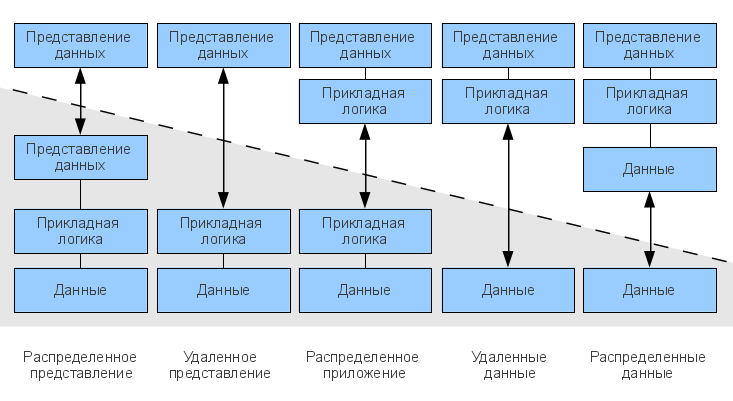
\includegraphics[width=0.75\textwidth]{cs-models}
\centering
\end{figure}

Cервер отвечает за управление рекламным инвентарем и объявлениями, сбор статистики показов, переходов и конверсий, поддержание внутренних инвариантов для сохранения актуальности и консистентности данных. Клиент отвечает за корректное отображение полученных от сервера рекламных материалов.

\section{Aрхитектура серверного приложения}

В качестве архитектуры серверного приложения используется трёхуровневая архитектура (англ. three-tier architecture) \cite{three-tier-architecture}, в которой разделяются функции представления, обработки и хранения данных. Разделяя приложение на уровни абстракции, появляется возможность внесения изменений в какой-то определённый слой, вместо того, чтобы перерабатывать всё приложение целиком. Трёхуровневая архитектура обычно состоит из слоя представления, слоя бизнес-логики и слоя доступа к данным.

\begin{figure}[h]
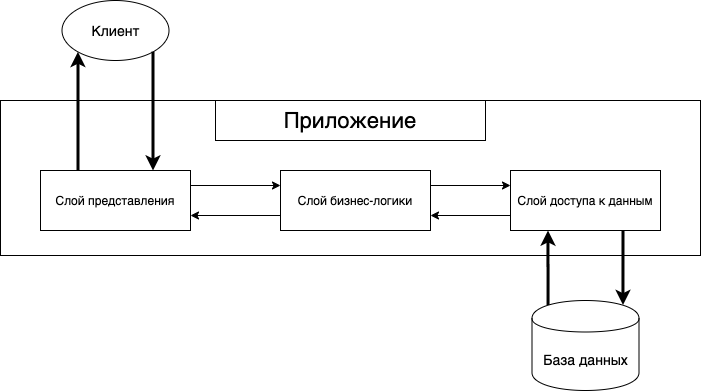
\includegraphics[width=0.75\textwidth]{three-tier-architecture}
\centering
\end{figure}

Перед тем как приступить к детальному описанию выбранной архитектуры, перечислим основные модели, которые представляют объекты предметной области, а затем последовательно рассмотрим каждый из слоев абстракции серверного приложения. 




\section{Модели}\label{sec:models}

\subsection{AdProvider}

 Модель AdProvider представляет поставщика товаров, из которых в последствии формируются рекламные объявления. Модель состоит из идентификатора провайдера, названия и ссылки на логотип для отображения ее в качестве небольшой иконки на объявлении, чтобы пользователь понимал с какой площадки представлен товар. В контексте данной работы Amazon единстенный поставщик.

\subsection{Ad}

Модель Ad представляет рекламное объявление и состоит из следующих полей:
\begin{itemize}
\item уникальный идентификатор объявления
\item идентификатор продукта
\item тип объявления 
\item контент объявления, представленный ссылками на изображения и видео, используемыми для отображения объявления на клиенте
\item ссылка для перехода по нажатию
\item идентификатор провайдера объявления
\item цена
\item категория
\end{itemize}

\textbf{Требования к форматам рекламных объявлений}
\begin{itemize}
	\item поддержка нативного формата (изображения с различными разрешениями + текст)
	\item поддержка баннерного формата (HTML разметка)
	\item поддержка видеоформата
\end{itemize}

\subsection{StrategyState}

Модель StrategyState представляет состояние стратегии таргетирования и состоит из следующих полей:
\begin{itemize}
\item идентификатор стратегии (одна из стратегий, описанных в \ref{sec:strategies})
\item идентификтор потока (подробнее описан в \ref{sec:strategies-state})
\item номер версии
\item набор пар (идентификатор объявления, скоринг объявления)
\end{itemize}

Ключ стратегии формируется из идентификатора стратегии, идентификатора потока и номера версии. Состояние стратегии предсталяет из себя набор пар идентификатор объявления и скоринг объявления, которые используются для задания порядка при запросе списка объявлений.

\subsection{Session}

Модель Session представляет сессию пользователя, запрашивающего рекламу из приложения. Данная модель связывает ключ сессии с ключем состояния стратегии.

\begin{figure}[h]
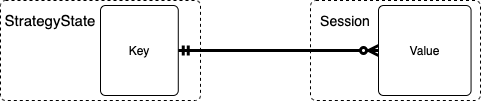
\includegraphics[width=0.75\textwidth]{strategy-state-session}
\centering
\end{figure}
Сохранение ключа состояния стратегии в сессии пользователя позволяет достичь консистентности списка объявлений при пагинации, как минимум, на время равное длительности одной сессии.

\subsection{Track, Impression, Click}

Модели Track, Impression и Click необходимы для представления данных статистики рекламных объявлений. Они хранят состояние на разных стадиях жизненного цикла объявления: 
\begin{itemize}
\item запрошено клиентом - создается экземпляр Track
\item пользователь увидел объявление - создается экземпляр Impression, связанный с уже созданным экземпляром Track
\item пользователь совершил переход по ссылке в объявлении - создается экземпляр Click, связанный с уже созданным экземпляром Track
\end{itemize}

\begin{figure}[h]

\includegraphics[width=0.75\textwidth]{track-impression-click}
\centering
\end{figure}

Все три модели имеют схожую сруктуру полей, используемых для расчета статистики по различным срезам:
\begin{itemize}
\item идентификатор трека
\item идентификатор рекламного объявления
\item идентификатор элемента рекламного инвентаря
\item идентификатор стратегии таргетинга
\item время создания
\end{itemize}

Модель Track еще дополнительно хранит обезличенные пользовательские данные отправляемые клиентским приложением во время запроса рекламы: тип и версия операционной системы, страна, язык, часовой пояс, версия клиентского приложения и др. Они используются в стратегиях таргетинга для увеличения вероятности клика на объявление.



\section{Слой доступа к данным}\label{sec:data-access-layer}

Слой доступа к данным (англ. data access layer) \cite{data-access-layer} взаимодействует только с вышестоящим слоем бизнес-логики и состоит из репозиториев. Репозиторий (англ. repository pattern) \cite{repository-pattern} обеспечивает абстракцию данных таким образом, что приложение может работать с простой абстракцией, интерфейс которой приближен к интерфейсу коллекции. Каждая модель обладает собственным репозиторием.

Добавление, удаление, обновление и получение элементов из этой коллекции выполняется с помощью ряда простых методов без необходимости решать проблемы с базами данных, такие как соединения, команды, курсоры. Использование этого шаблона позволяет добиться слабой связности и отсутствию зависимости от способа хранения данных. Таким образом вся логика необходимая для функционирования моделей содержится в репозиториях.

Исходя из представленных моделей \ref{sec:models} и требований к рекламному серверу репозитории делятся на три группы:
\begin{itemize}
\item репозиторий модели рекламного объявления
\item репозитории моделей таргетинга
\item рапозитории моделей трекинга
\end{itemize}

Также слой доступа к данным состоит из кэша рекламных объявлений. Он необходим для сокращения времени ответа на запросы рекламы, а также существенно снижает количество обращений к базе данных.

\section{Слой бизнес-логики}\label{sec:business-logic-layer}

Слой бизнес-логики взаимодействует низлежащим слоем доступа к данным и с вышестоящим слоем представления. Состоит из модулей, которые должны быть слабосвязанными между собой для того, чтобы внесение изменений в один или несколько модулей не затрагивало весь код приложения.

Модуль - это высокоуровневый компонент системы, взаимодействующий с другими модулями, а также с репозиториями . При разделении бизнес-логики на модули используется подход SOLID \cite{SOLID}, который обеспечивает высокую гибкость, изменяемость и поддерживаемость кода.

Далее рассмотрим каждый модуль по отедельности с указаением его назначения, алгоритма работы и диаграмм для наглядности.

\subsection{Обновление объявлений}

Обновление рекламный объявлений является автоматическим и в контексте нашего сервиса выполняет функцию рекламодателя, т.к. генерирует объявления. 

\begin{figure}[h]

\includegraphics[width=0.75\textwidth]{ad-updater}
\centering
\end{figure}
Стадии данного процеса описываются следующим алгоритмом:
\begin{enumerate}
\item отбор актуальных товаров на Amazon по заранее заданным критериям
\item генерация рекламных объявлений на основе полученных товаров
\item сохранение полученных объявлений в базе данных
\item деактивация уже существующих в системе объявлений и активация только что созданных
\item обновление объявлений в кэше
\end{enumerate}

При обновлении объявлений в основной базе данных необходимо также обновить их и в кэше, т.к. кэш не является долгосрочным хранилищем, а лишь ускоряет доступ к актуальной версии объявлений. Выполнение обновления объявлений происходит по расписанию, установленному для соблюдения требуемого уровня актуальности.

\subsection{Обновление категорий интереса пользователя}

 У каждого пользователя категории, которые его инетерсуют более остальных. Выделив подобные категории можно показывать ему объявления наиболее релевантные интересам пользователя. Данный подход позволит увеличить средний CTR, что является позитивным фактором как для пользователя, который видит только интересующую его рекламу, так и для рекламодателя с издателем, которые извлекают дополнительную прибыль.
 
 Выделение категорий интереса пользователя происходит на основе анализа посещенных веб-страниц. Каждой странице на основе алгоритмов машинного обучения сопоставляется список категорий, наиболее релевантных данной странице. Для каждого пользователя хранится вектор пар категорий и соответствующее количество посещений веб-страниц по данной категории за 30 дней. Схожим образом для каждого пользователя подсчитывается еще один вектор пар категорий рекламных объявлений и количество переходов по объявлениям данной категории за 30 дней.
 
Отсортировав каждый из двух полученных векторов по невозрастанию количества посещений / переходов  и выбрав первые 5 категорий в каждом, получим два профиля краткосрочных интересов пользователя, которые теперь можно использовать в таргетинге.

\subsection{Таргетинг}

Таргетинг - механизм подбора рекламного объявления для показа пользователю таким образом, чтобы вероятность перехода по нему была максимальной.

\begin{figure}[h]
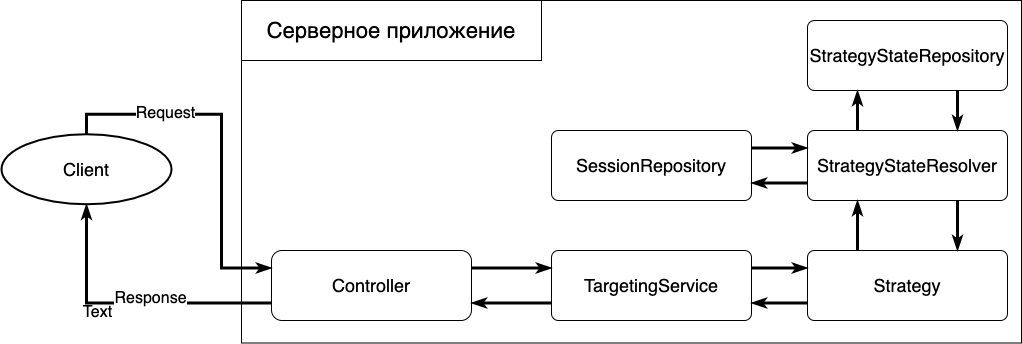
\includegraphics[width=0.75\textwidth]{targeting-process}
\centering
\end{figure}

В рамках данной работы алгоритм таргетинга состоит из следующих этапов:
\begin{itemize}
\item фильтрация всех доступных объявлений на основе параметров запроса и пользователя
\item для каждого товара одно объявление с наивысшим CTR
\item определение каждого объявления в одну из трех групп testing, rejected, approved на основе числе показов и CTR
\item ранжирование по группам в порядке approved, testing, rejected
\item ранжирование внутри группы по CTR
\item получение одного или нескольких объявлений из итогового списка
\end{itemize}

Стратегия таргетинга - реализация вышепреведенного алгоритма с применением конкретных подходов для фильтрации, ранжирования и выбора рекламных объявлений. Для каждой стратегии формируется свой набор отранжированных списков объявлений и сохраняется в кэш, чтобы ускорить процесс получения объявлений. Выбор того или иного списка определяется логикой стратегии, а также параметрами пользователя, запрашивающего объявления. 

Каждая стратегия таргетирования назначает веса рекламным объявлениям \ref{creative-sequencing}, чтобы управлять их частотой показа. Три группы объявлений (нарисовать автомат переходов): testing, rejected, approved. Рандомизация применяется для равномерного выбора объявлений. 

Выбор оптимальной стратегии на основе данных, представленных в запросе: если рекламное объявление должно зависеть от контекста, в котором оно будет показано выбирается одна из стратегий, которая таргетирует на основании параметров переданного контекста. Иначе выбирается стратегия, которая таргетирует на основании накопленных знаниях о категориях интереса текущего пользователя.

\subsection{Стратегии таргетинга}\label{sec:strategies}

Любая стратегия должна соответствовать следующим требованиям

\textbf{Требования к показу единичных объявлений:}
\begin{itemize}
	\item возможность задания категории объявления
	\item возможность задания списка стран, в которых будет показано объявление
\end{itemize}

\textbf{Требования к показу списка объявлений:}
\begin{itemize}
	\item консистентность списка для пользователя / конкретного девайса пользователя
	\item возможность фильтрации провайдеров / товаров?
	\item возможность учета для каждого товара из списка: показов и кликов
\end{itemize}

Предлагается 4 стратегии различающихся по ...

\textbf{Для таргетирования используются 4 стратегии}:
\begin{enumerate}
	\item случайные объявления
	\item объявления с глобально высоким показателем CTR
	\item объявления с высоким показателем CTR в категориях интереса данного пользователя, рассчитанных на основе просмотренных страниц в интернете
	\item объявления с высоким показателем CTR в категориях интереса данного пользователя, рассчитанных на основе кликов по объявлениям внутри приложения
\end{enumerate}

Расписать принцип работы каждой из 4-х стратегий: матчинг категорий - random (стратегия создавалась для быстрого получения MVP), по кликам overall, по просмотрам страниц (IBM Watson NLP), по кликам на объявления (Категории товаров Amazon)

\subsection{Состояния стратегий}\label{sec:strategies-state}

\textbf{StrategyState threads} - обновление состояний потока по расписанию

\textbf{StrategyState resolving} - использует структурный шаблон проектирования Flyweight для уменьшения потребления оперативной памяти для хранения большого сессий. (sessionKey по идее может быть произвольной строкой предоставляемой Publisher'ом)

TODO

\subsection{Трекинг показов и переходов}

Трекинговая закрытая воронка (Track / Impression / Click)

\begin{figure}[h]
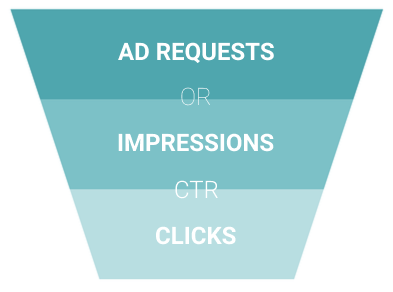
\includegraphics[width=0.5\textwidth]{funnel}
\centering
\end{figure}

Сценарии использования накопленных данных трекинга:
\begin{itemize}
	\item расчет статистики по рекламным объявлениям: Impressions, Clicks, Conversions, CTR, CR для отображение в панели рекламодателя
	\item использование CTR рекламного объявления в стратегиях таргетинга
	\item оптимизация бизнес-процесса на основе данных (Data-driven decision making)
	\item автоматический выбор стратегии таргетирования на основе статистики стратегий
\end{itemize}

\subsection{Статистика по объявлениям и стратегиям}

\textbf{Требования к аналитике:}
\begin{itemize}
	\item возможность просмотра статистики каждого рекламного объявления в формате (AdId, Показы, Клики, CTR, тут колонки таблицы) с фильтрацией по … и группировкой по …
	\item возможность просмотра параметров эффективности (OR, CTR) стратегий таргетинга, рассчитанных по данным трекинга, с фильтрацией по интервалу дат и группировкой по идентификатору стратегии
\end{itemize}


\section{Сценарии использования}

Слой клиента представляет из себя контракт взаимодействия клиента и сервера. Получение данных клиентом подразумевает отправку HTTP запросов  на сервер в установленном формате и с токеном для подтверждения доступа. Среди всех сценариев можно выделить два типа триггеров: запрос к серверу, запуск по расписанию в контексте задачи.

Далее рассмотрим совместное функционирование приведенных модулей в основных сценариях использования.

\subsection{Получение одного объявления}

Получение данных пользователя. 
Выбор стратегии таргетинга. 
Получение списка объявлений по выбранной стратегии.

\subsection{Получение списка объявлений}

Получение данных пользователя и текущей сессии (у каждой сессии свой уникальный ключ). 
Выбор стратегии таргетинга. 
Получение списка объявлений по выбранной стратегии.

\subsection{Трекинг показов и переходов}

TODO

\subsection{Получение статистики по стратегиям таргетинга}

TODO

\chapterconclusion

TODO






\chapter{Техническая реализация и внедрение предложенной архитектуры}

Итоговая архитектура рекламной сети: инфраструктура, количество серверов, тип масштабирования, базы данных, кэширование...

Текущая инфраструктура компании - это несколько Kubernetes кластеров. Серверные приложения являются микросервисами, которые общаются по AMQP. Разделение на микросервисы по функциональному принципу. 

Ad server - это еще один микросервис в инфраструктуре компании. Также как и для остальных микросервисов для данного рекламного сервера была выбрана платформа Node.js.

Выбран язык программирования Typescript \cite{typescript-lang} версии 3.8. Основные преимущества данного языка:
\begin{itemize}
\item широко используется в различных проектах компании (уменьшает порог вхождения членов команды)
\item современный язык, разработанный компанией Microsoft (гарантирует надежность и развитие языка)
\item обладает возможностью писать как в императивном стиле так и декларативном (позволяет повысить читаемость кода и использовать функциональный стиль программирования)
\item обладает строгой типизацией (позволяет существенно сократить вероятность появления дефектов в процессе разработки и сопровождения кода)
\end{itemize}

\section{Процесс разработки}

Процесс разработки - циклы разработки, состоящие из следующих стадий (Scrum):
\begin{itemize}
	\item сформировать требования
	\item спроектировать
	\item реализовать на основе требований и модели архитектуры
	\item протестировать
	\item внедрить
\end{itemize}

Готовые модули, используемые в проекта, находятся в реестре публичных Node.js модулей - NPM (ссылка)

Используем Git (git-flow / GitHub-flow), Bitbucket (pull-requests, code-review)

\section{Инфраструктура}

Описать кластер в Google Kubernetes Engine. Хранение изображений в Google Buckets. Также работает как CDN

\section{Конфигурация, окружение}

Множество окружений: staging, production \cite{twelve-factor-app}

\section{Аутентификация запросов}

Аутентификация: JWT

\section{Работа с моделями}

\subsection{Модель Ad}

Модель Ad состоит из сущностей Ad, AdMedia, Price (отношения one-to-many). Для хранения этих сущностей используется база данных MongoDB \cite{mongodb} (почему? т.к. база общего назначение + является основной в компании, позволяет относительно безболезненно вносить изменения в схему данных)

\subsection{Модели трекинга}

Track, Impression, Click (ClickHouse, т.к. нужна поддержка OLAP)

\subsection{ORM}

Выбор ORM и драйверов для работы с БД: какие выбраны и почему?



\section{Обновление объявлений (AdUpdater)}

Так как объявления формируются на основе товаров с Amazon, то для начала нам надо определиться какие именно товары мы хотим показывать нашим пользователям.

\subsection{Критерии отбора товаров}

\subsection{Получение товаров через Product Advertising API}

На данный момент официальным и актуальным способов доступа к товарам, размещаемым на площадке Amazon является интерфейс Product Advertising API 5.0 \cite{amazon-paapi-docs}. Доступ к API осуществляется с помощью access-token. Соединение происходит по HTTP протоколу, формат запросов и ответов - JSON. Для осуществеления авторизованных запросов используется Node.js SDK \cite{amazon-paapi-sdk}

В ссылку на товар подставляется \textit{PartnerTag} для связывания покупок, совершаемых по данной ссылке, с партнером, который привел покупателя.

\subsection{Создание объявления}

Как мы расфасовываем Resource по сущностям Ad, AdMedia, Price.

\textbf{Обновление Price}

Заменяем текущее значение модели Price связанной с Ad на новое

\textbf{Обновление AdMedia}

При обновлении Ad уникализируем связанные с ним AdMedia по url, чтобы не плодить кучу копий со статусом enabled = false в базе.


Оборачивание ссылки с помощью RedirectEncoder для отслежвания переходов. (переместить в контроллер!)



\section{Кэширование объявлений (AdService + AdCache)}

Обновление объявлений, описанное в предыдушей подглаве, инициирует обновления кэша объявлений для сохранения консистентности. Это важно так как 
Кэш объявлений и скоринга. Redis, т.к. нужен быстрый доступ к объявлениям) . Обосновать выбор той или иной базы для каждой сущности, желательно найти бенчмарки сравнения MongoDB и Redis)

\section{Обновление состояний стратегий (StrategyStateUpdater)}

Каждое состояние рассчитывается и сохраняется для последующих обращений в Redis , так как расчитывать весь список объявлений на каждый запрос к существенному увеличению времени ответа, а также абсолютно чрезмерному и неоправданному использованию серверных мощностей.

(Amazon <-> IBM Watson category mapper)

\section{Контроллеры}

Для обработки запросов, поступающих к нашему микросервису, используется фреймворк Koa2 (ссылка), работающий поверх веб-сервера Node.js (ссылка).

Контроллер реализуется посредством использования класса "middleware" (который является примером поведенческого паттерна проектирование Chain of Responsibility)

Список контроллеров, по каждому входные параметры и выходные параметры (объемные ответы в виде ссылок на примечание)

\section{Документация}

Документация openapi.yml


\section{Тестирование}

\subsection{Концепция написания тестов}

Процесс тестирования полученной платформы: Unit/Integration/Functional/E2E тестирование, White-box/Black-box, в каком количестве? для проверки чего и какие виды тестов использовались?

Вставки с кодом тестов для иллюстрации фреймфорка: сетап-действие-ассерт (https://bitbucket.org/fulldivevr/community-doc/src/master/tdd-conspect.md)

\subsection{Локальное тестирование}

Как производится локальное тестирование не-unit тестов: Docker, docker-compose

Команды для запуска тестирования в package.json: test:unit, test:e2e и т.д. (mocha, chai)

\subsection{Нагрузочное тестирование}

количественные параметры (количество показов, кликов в секунду / сутки, максимальное количество ошибок за сутки / месяц)
время ответа на 95 процентиле (P95) не более 200 мс

\section{Внедрение}

Процесс внедрения (развертывания): , описание *.yaml файлов конфигурации, helm-charts, skaffold; BitBucket pipelines; Terraform; тэги и версионирование

\chapterconclusion

Вывод в конце третьей главы





%% Макрос для заключения. Совместим со старым стилевиком.
\startconclusionpage

Дальнейшее развитие (стратегические направления / цели) (исходя из них можно уточнить требования к реализации платформ
(все дальнейшие разработки и улучшения также направлены на увеличение прибыли (согласно основному бизнес-процессу итоговая цель - прибыль))

N1 Развитие компании в качестве своего собственного рекламодателя (growth as Advertiser / Ad provider). Как это сделать?
\begin{itemize}
\item Идея 1: увеличить количество исходных рекламодателей - интегрировать E-commerce платформы Ebay, Aliexpress, Wildberries, …
\item Идея 2: подбирать множество товаров таким образом, чтобы итоговое число покупок было максимально (слишком мало товаров - неудовлетворенный спрос, слишком много товаров - проблема выбора и рассеивание внимания)
\item Идея 3: тиражирование товаров с максимально высокой вероятностью покупки для конкретного пользователя, например, товары из интересующих пользователя категорий (персонализация показываемой рекламы)
\end{itemize}

N2 Оптимизация количества и качества плейсментов внтури приложений компании (growth as Publisher)

N3 Привлечение сторонних рекламодателей (добавление RTB / Bidders)

N4 Добавление стратегий основанных на контекстном таргетинге

\printmainbibliography

%% После этой команды chapter будет генерировать приложения, нумерованные русскими буквами.

\appendix

\chapter{Графики}\label{sec:app:1}

TODO

\chapter{Примеры ответов на запросы}\label{sec:app:2}

Примеры запросов и ответов API (ad, ads)

\chapter{Категории товаров на Amazon}\label{sec:app:3}

TODO

\chapter{Реклама в приложении Fulldive Browser на Android}\label{sec:app:4}

Скрини одиночных объявлений (лента, страница) + products feed

\end{document}